\documentclass[]{article}
\usepackage{lmodern}
\usepackage{amssymb,amsmath}
\usepackage{ifxetex,ifluatex}
\usepackage{fixltx2e} % provides \textsubscript
\ifnum 0\ifxetex 1\fi\ifluatex 1\fi=0 % if pdftex
  \usepackage[T1]{fontenc}
  \usepackage[utf8]{inputenc}
\else % if luatex or xelatex
  \ifxetex
    \usepackage{mathspec}
  \else
    \usepackage{fontspec}
  \fi
  \defaultfontfeatures{Ligatures=TeX,Scale=MatchLowercase}
\fi
% use upquote if available, for straight quotes in verbatim environments
\IfFileExists{upquote.sty}{\usepackage{upquote}}{}
% use microtype if available
\IfFileExists{microtype.sty}{%
\usepackage{microtype}
\UseMicrotypeSet[protrusion]{basicmath} % disable protrusion for tt fonts
}{}
\usepackage[margin=1in]{geometry}
\usepackage{hyperref}
\hypersetup{unicode=true,
            pdftitle={hw4},
            pdfauthor={Jess Kaminsky},
            pdfborder={0 0 0},
            breaklinks=true}
\urlstyle{same}  % don't use monospace font for urls
\usepackage{color}
\usepackage{fancyvrb}
\newcommand{\VerbBar}{|}
\newcommand{\VERB}{\Verb[commandchars=\\\{\}]}
\DefineVerbatimEnvironment{Highlighting}{Verbatim}{commandchars=\\\{\}}
% Add ',fontsize=\small' for more characters per line
\usepackage{framed}
\definecolor{shadecolor}{RGB}{248,248,248}
\newenvironment{Shaded}{\begin{snugshade}}{\end{snugshade}}
\newcommand{\KeywordTok}[1]{\textcolor[rgb]{0.13,0.29,0.53}{\textbf{{#1}}}}
\newcommand{\DataTypeTok}[1]{\textcolor[rgb]{0.13,0.29,0.53}{{#1}}}
\newcommand{\DecValTok}[1]{\textcolor[rgb]{0.00,0.00,0.81}{{#1}}}
\newcommand{\BaseNTok}[1]{\textcolor[rgb]{0.00,0.00,0.81}{{#1}}}
\newcommand{\FloatTok}[1]{\textcolor[rgb]{0.00,0.00,0.81}{{#1}}}
\newcommand{\ConstantTok}[1]{\textcolor[rgb]{0.00,0.00,0.00}{{#1}}}
\newcommand{\CharTok}[1]{\textcolor[rgb]{0.31,0.60,0.02}{{#1}}}
\newcommand{\SpecialCharTok}[1]{\textcolor[rgb]{0.00,0.00,0.00}{{#1}}}
\newcommand{\StringTok}[1]{\textcolor[rgb]{0.31,0.60,0.02}{{#1}}}
\newcommand{\VerbatimStringTok}[1]{\textcolor[rgb]{0.31,0.60,0.02}{{#1}}}
\newcommand{\SpecialStringTok}[1]{\textcolor[rgb]{0.31,0.60,0.02}{{#1}}}
\newcommand{\ImportTok}[1]{{#1}}
\newcommand{\CommentTok}[1]{\textcolor[rgb]{0.56,0.35,0.01}{\textit{{#1}}}}
\newcommand{\DocumentationTok}[1]{\textcolor[rgb]{0.56,0.35,0.01}{\textbf{\textit{{#1}}}}}
\newcommand{\AnnotationTok}[1]{\textcolor[rgb]{0.56,0.35,0.01}{\textbf{\textit{{#1}}}}}
\newcommand{\CommentVarTok}[1]{\textcolor[rgb]{0.56,0.35,0.01}{\textbf{\textit{{#1}}}}}
\newcommand{\OtherTok}[1]{\textcolor[rgb]{0.56,0.35,0.01}{{#1}}}
\newcommand{\FunctionTok}[1]{\textcolor[rgb]{0.00,0.00,0.00}{{#1}}}
\newcommand{\VariableTok}[1]{\textcolor[rgb]{0.00,0.00,0.00}{{#1}}}
\newcommand{\ControlFlowTok}[1]{\textcolor[rgb]{0.13,0.29,0.53}{\textbf{{#1}}}}
\newcommand{\OperatorTok}[1]{\textcolor[rgb]{0.81,0.36,0.00}{\textbf{{#1}}}}
\newcommand{\BuiltInTok}[1]{{#1}}
\newcommand{\ExtensionTok}[1]{{#1}}
\newcommand{\PreprocessorTok}[1]{\textcolor[rgb]{0.56,0.35,0.01}{\textit{{#1}}}}
\newcommand{\AttributeTok}[1]{\textcolor[rgb]{0.77,0.63,0.00}{{#1}}}
\newcommand{\RegionMarkerTok}[1]{{#1}}
\newcommand{\InformationTok}[1]{\textcolor[rgb]{0.56,0.35,0.01}{\textbf{\textit{{#1}}}}}
\newcommand{\WarningTok}[1]{\textcolor[rgb]{0.56,0.35,0.01}{\textbf{\textit{{#1}}}}}
\newcommand{\AlertTok}[1]{\textcolor[rgb]{0.94,0.16,0.16}{{#1}}}
\newcommand{\ErrorTok}[1]{\textcolor[rgb]{0.64,0.00,0.00}{\textbf{{#1}}}}
\newcommand{\NormalTok}[1]{{#1}}
\usepackage{graphicx,grffile}
\makeatletter
\def\maxwidth{\ifdim\Gin@nat@width>\linewidth\linewidth\else\Gin@nat@width\fi}
\def\maxheight{\ifdim\Gin@nat@height>\textheight\textheight\else\Gin@nat@height\fi}
\makeatother
% Scale images if necessary, so that they will not overflow the page
% margins by default, and it is still possible to overwrite the defaults
% using explicit options in \includegraphics[width, height, ...]{}
\setkeys{Gin}{width=\maxwidth,height=\maxheight,keepaspectratio}
\IfFileExists{parskip.sty}{%
\usepackage{parskip}
}{% else
\setlength{\parindent}{0pt}
\setlength{\parskip}{6pt plus 2pt minus 1pt}
}
\setlength{\emergencystretch}{3em}  % prevent overfull lines
\providecommand{\tightlist}{%
  \setlength{\itemsep}{0pt}\setlength{\parskip}{0pt}}
\setcounter{secnumdepth}{0}
% Redefines (sub)paragraphs to behave more like sections
\ifx\paragraph\undefined\else
\let\oldparagraph\paragraph
\renewcommand{\paragraph}[1]{\oldparagraph{#1}\mbox{}}
\fi
\ifx\subparagraph\undefined\else
\let\oldsubparagraph\subparagraph
\renewcommand{\subparagraph}[1]{\oldsubparagraph{#1}\mbox{}}
\fi

%%% Use protect on footnotes to avoid problems with footnotes in titles
\let\rmarkdownfootnote\footnote%
\def\footnote{\protect\rmarkdownfootnote}

%%% Change title format to be more compact
\usepackage{titling}

% Create subtitle command for use in maketitle
\newcommand{\subtitle}[1]{
  \posttitle{
    \begin{center}\large#1\end{center}
    }
}

\setlength{\droptitle}{-2em}
  \title{hw4}
  \pretitle{\vspace{\droptitle}\centering\huge}
  \posttitle{\par}
  \author{Jess Kaminsky}
  \preauthor{\centering\large\emph}
  \postauthor{\par}
  \predate{\centering\large\emph}
  \postdate{\par}
  \date{April 9, 2018}


\begin{document}
\maketitle

\subsection{Question 1}\label{question-1}

\subsubsection{Part A}\label{part-a}

In exploring the risky behavior dataset, we hope to find a model that
best predicts the number of unprotected sex acts among couples and the
efficacy of an intervention the provided counseling sessions regarding
practices that could reduce their likelihood of contracting HIV. When
initially exploring the variables of interest - number of unprotected
sex acts - by treatment group, we see that there are some potential
outliers in the women alone and control groups - especially for baseline
sex acts; however if these larger data points were excluded, the
distribution of sex acts at baseline seem approximately equal among
treatment groups. We can see a decrease in mean of the outcome at follow
up among all treatment groups, but most notably in the women alone and
couples groups - even the potential outliers decreased markedly. From
exploring the following boxplots, there is evidence that the
intervention was succesful at reducing the number of unprotected sex
acts. We will further explore this relationship using poisson
regression.

\begin{Shaded}
\begin{Highlighting}[]
\CommentTok{#convert 2 treatment dummy vars to 1 treatment variable that also accounts for contol group - this variable is the number of partners that received counseling}
\KeywordTok{par}\NormalTok{(}\DataTypeTok{mfrow=}\NormalTok{(}\KeywordTok{c}\NormalTok{(}\DecValTok{2}\NormalTok{,}\DecValTok{2}\NormalTok{)))}
\KeywordTok{boxplot}\NormalTok{(bupacts~treatment, }\DataTypeTok{names =} \KeywordTok{c}\NormalTok{(}\StringTok{"Control"}\NormalTok{, }\StringTok{"Women Alone"}\NormalTok{, }\StringTok{"Couples"}\NormalTok{), }\DataTypeTok{main =} \StringTok{"Baseline Sex Acts by Treatment Group"}\NormalTok{, }\DataTypeTok{ylab =} \StringTok{"Number of Unprotected Sex Acts"}\NormalTok{, }\DataTypeTok{data =} \NormalTok{risky)}
\KeywordTok{boxplot}\NormalTok{(fupacts~treatment, }\DataTypeTok{names =} \KeywordTok{c}\NormalTok{(}\StringTok{"Control"}\NormalTok{, }\StringTok{"Women Alone"}\NormalTok{, }\StringTok{"Couples"}\NormalTok{), }\DataTypeTok{main =} \StringTok{"Follow-Up Sex Acts by Treatment Group"}\NormalTok{, }\DataTypeTok{ylab =} \StringTok{"Number of Unprotected Sex Acts"}\NormalTok{, }\DataTypeTok{ylim =} \KeywordTok{c}\NormalTok{(}\DecValTok{0}\NormalTok{, }\DecValTok{300}\NormalTok{))}
\end{Highlighting}
\end{Shaded}

\includegraphics{hw4_files/figure-latex/unnamed-chunk-1-1.pdf}

The following model is the result of fitting a generalized linear model
with poisson regression modeling the number of unprotected sex acts at
followup as a function of treatment group. Here we are using
women\_alone and couples as indicator variables for two of the three
treatment groups - if both indicator variables are equal to 0 the
subject is in the control group where neither partner has received
counseling.

\(log(Unprotected Sex Acts_{follow-up}) = 3.09 - 0.322(Couples = 1) - 0.572(Women Alone = 1)\)
\(Unprotected Sex Acts_{follow-up} = e ^ {3.09 - 0.322(Couples = 1) - 0.572(Women Alone = 1)}\)

A summary of the model is presented below.

\begin{Shaded}
\begin{Highlighting}[]
\KeywordTok{summary}\NormalTok{(model_a)}
\end{Highlighting}
\end{Shaded}

\begin{verbatim}
## 
## Call:
## glm(formula = fupacts ~ couples + women_alone, family = poisson, 
##     data = risky)
## 
## Deviance Residuals: 
##     Min       1Q   Median       3Q      Max  
## -6.6285  -4.9794  -3.2015   0.9847  27.1502  
## 
## Coefficients:
##              Estimate Std. Error z value Pr(>|z|)    
## (Intercept)   3.08960    0.01901  162.55   <2e-16 ***
## couples1     -0.32243    0.02737  -11.78   <2e-16 ***
## women_alone1 -0.57212    0.03023  -18.93   <2e-16 ***
## ---
## Signif. codes:  0 '***' 0.001 '**' 0.01 '*' 0.05 '.' 0.1 ' ' 1
## 
## (Dispersion parameter for poisson family taken to be 1)
## 
##     Null deviance: 13299  on 433  degrees of freedom
## Residual deviance: 12925  on 431  degrees of freedom
## AIC: 14256
## 
## Number of Fisher Scoring iterations: 6
\end{verbatim}

Based on this model, we can interpret that the estimated number of
unprotected sex acts per three months for those in the control group is
21.977. The expected number of unprotected sex acts at follow-up for
those in the couples treatment group is \(e^{3.09-0.322(1)}= 15.927\)
per 3 months and \(e^{3.09-0.572(1)} = 12.404\) per 3 months for those
in the the women alone treatment group. Subjects in the couples group
will have unprotected sex at a rate that is (\(e^{-0.322}=0.725\)) =
72.5\% less than those in the control group. Subjects in the women alone
will have unprotected sex at a rate that is (\(e^{-0.572}=0.564\)) =
56.4\% less than those in the control group.

In order to assess the fit of this model, we will perform a chi-squared
test, testing the null hypothesis test that the ratio betweel the model
residual deviance and residual degrees of freedm is equal to 1, we
obtain a p-value that is approximately 0. Therefore, we can conclude
that the ratio is significantly different than 1 which provides us with
evidence that the model does not fit well and there is evidence of
dispersion.

To further examine the dispersion of this model, we will conduct an
overdispersion hypothesis test to test the following hypotheses, where k
is the dispersion parameter: \$H\_0: k = 1 \$ \$H\_1: k \textgreater{} 1
\$

\begin{Shaded}
\begin{Highlighting}[]
\KeywordTok{dispersiontest}\NormalTok{(model_a, }\DataTypeTok{alternative =} \StringTok{"greater"}\NormalTok{)}
\end{Highlighting}
\end{Shaded}

\begin{verbatim}
## 
##  Overdispersion test
## 
## data:  model_a
## z = 4.7542, p-value = 9.961e-07
## alternative hypothesis: true dispersion is greater than 1
## sample estimates:
## dispersion 
##    43.8295
\end{verbatim}

With a p-value = 9.961e-07, there is strong evidence to conclude that
the true dispersion parameter is significantly greater than 1 and there
is overdispersion in this model.

\subsubsection{Part B}\label{part-b}

We will now extend the above model and include the other predictors
included in the dataset - sex, baseline HIV status, and baseline number
of unprotected sex acts. Poisson regression generated the following
model.

\$log(Unprotected Sex Acts\_\{follow-up\}) = 2.787 + 0.109(sex = woman)
- 0.410(Couples = 1) - 0.662(Women Alone = 1) - 0.438(Baseline HIV = +)
+ 0.011(Baseline Sex Acts) \$
\(Unprotected Sex Acts_{follow-up} = e ^ {2.787 + 0.109(sex = woman) - 0.410(Couples = 1) - 0.662(Women Alone = 1) - 0.438(Baseline HIV = +) + 0.011(Baseline Sex Acts)}\)

A summary of the model is presented below.

\begin{Shaded}
\begin{Highlighting}[]
\NormalTok{model_b <-}\StringTok{ }\KeywordTok{glm}\NormalTok{(fupacts ~}\StringTok{ }\NormalTok{., }\DataTypeTok{family =} \NormalTok{poisson, }\DataTypeTok{data =} \NormalTok{risky[-}\DecValTok{7}\NormalTok{])}
\KeywordTok{summary}\NormalTok{(model_b)}
\end{Highlighting}
\end{Shaded}

\begin{verbatim}
## 
## Call:
## glm(formula = fupacts ~ ., family = poisson, data = risky[-7])
## 
## Deviance Residuals: 
##     Min       1Q   Median       3Q      Max  
## -18.679   -4.305   -2.511    1.368   23.361  
## 
## Coefficients:
##                  Estimate Std. Error z value Pr(>|z|)    
## (Intercept)     2.7871257  0.0235599 118.300  < 2e-16 ***
## sexwoman        0.1086694  0.0237301   4.579 4.66e-06 ***
## couples1       -0.4099761  0.0282298 -14.523  < 2e-16 ***
## women_alone1   -0.6622159  0.0308962 -21.434  < 2e-16 ***
## bs_hivpositive -0.4383170  0.0353804 -12.389  < 2e-16 ***
## bupacts         0.0107789  0.0001738  62.013  < 2e-16 ***
## ---
## Signif. codes:  0 '***' 0.001 '**' 0.01 '*' 0.05 '.' 0.1 ' ' 1
## 
## (Dispersion parameter for poisson family taken to be 1)
## 
##     Null deviance: 13299  on 433  degrees of freedom
## Residual deviance: 10200  on 428  degrees of freedom
## AIC: 11537
## 
## Number of Fisher Scoring iterations: 6
\end{verbatim}

From the model, we can interpret that the estimated number of
unprotected sex acts per three months for HIV negative males in the
control group having 0 unprotected sex acts at baseline is 2.787. As
another example, the estimated count of the outcome per three months for
a HIV negative female in the couples group with 10 unprotected sex acts
would be calculated as follows:
\(e ^ {2.787 + 0.109(1) - 0.410(1) - 0.662(0) - 0.438(0) + 0.011(10)} = 13.410\)
unprotected sex acts at followup per three months

We can interpret the coefficients of the model as follows: - The
predicted count of unprotected sex acts at follow-up per three months
for women is (\(e^{0.109}=1.115\)) = 11.5\% greater than the rate for
men when holding all other predictors constant. - The predicted count of
unprotected sex acts at follow-up per three months for subjects who are
HIV positive at baseline is (\(e^{-0.438}=0.645\)) = 64.5\% less than
the expected number for those who are HIV negative at baseline while
holding all other predictors constant. - The predicted count of
unprotected sex acts at follow-up per three months increases by
(\(e^{0.011}=1.011\)) = 1.1\% for every 1 unit increase in number of
unprotected sex acts at baseline.

We will asses the fit of this model with a chi-squared test, testing the
null hypothesis test that the ratio betweel the model residual deviance
and residual degrees of freedm is equal to 1, we obtain a p-value that
is approximately 0. We can conclude that the ratio is significantly
different than 1 which provides us with evidence that the model does not
fit well and there is evidence of dispersion. The residual deviance for
this model is 10200 indicating a slightly better fit than the previous
model where the residual deviance was 12925.

In order to test for overdispersion in this model, we will test the
following hypotheses:

\$H\_0: k = 1 \$ \$H\_1: k \textgreater{} 1 \$

With a p-value = 1.282e-08, there is strong evidence to conclude that
the true dispersion parameter is significantly greater than 1. There is
even stronger evidence of overdispersion in this model compared to the
previous model.

\begin{Shaded}
\begin{Highlighting}[]
\KeywordTok{dispersiontest}\NormalTok{(model_b, }\DataTypeTok{alternative =} \StringTok{"greater"}\NormalTok{)}
\end{Highlighting}
\end{Shaded}

\begin{verbatim}
## 
##  Overdispersion test
## 
## data:  model_b
## z = 5.5689, p-value = 1.282e-08
## alternative hypothesis: true dispersion is greater than 1
## sample estimates:
## dispersion 
##   29.65146
\end{verbatim}

\subsubsection{Part C}\label{part-c}

We will now fit an overdispersed Poisson model using the quasipoisson
because the 2 preceeding models showed significant evidence of
overdispersion. The second model - using all variables as predictors -
had a better fit than the simpler model, therefore we will use all
predictors. Using the quasipoisson family, the following model was
generated:

\$log(Unprotected Sex Acts\_\{follow-up\}) = 2.787 + 0.109(sex = woman)
- 0.410(Couples = 1) - 0.662(Women Alone = 1) - 0.438(Baseline HIV = +)
+ 0.011(Baseline Sex Acts) \$
\(Unprotected Sex Acts_{follow-up} = e ^ {2.787 + 0.109(sex = woman) - 0.410(Couples = 1) - 0.662(Women Alone = 1) - 0.438(Baseline HIV = +) + 0.011(Baseline Sex Acts)}\)

When fitting a quasi-poisson model, the coefficients do not change,
however the standard errors and therefore p-values for each term do
change. In this previous model, all coefficients were sigificant
predictors of the outcome. In this model, the indicator variable for
women is not significant in predicting the count of unprotected sex acts
over a three month period. All other variables in the model are still
significant after adjusting for overdispersion. A summary of the model
is presented below.

\begin{Shaded}
\begin{Highlighting}[]
\NormalTok{model_b2 <-}\StringTok{ }\KeywordTok{glm}\NormalTok{(fupacts ~}\StringTok{ }\NormalTok{., }\DataTypeTok{family =} \NormalTok{quasipoisson, }\DataTypeTok{data =} \NormalTok{risky[-}\DecValTok{7}\NormalTok{])}
\KeywordTok{summary}\NormalTok{(model_b2)}
\end{Highlighting}
\end{Shaded}

\begin{verbatim}
## 
## Call:
## glm(formula = fupacts ~ ., family = quasipoisson, data = risky[-7])
## 
## Deviance Residuals: 
##     Min       1Q   Median       3Q      Max  
## -18.679   -4.305   -2.511    1.368   23.361  
## 
## Coefficients:
##                  Estimate Std. Error t value Pr(>|t|)    
## (Intercept)     2.7871257  0.1290515  21.597  < 2e-16 ***
## sexwoman        0.1086694  0.1299838   0.836 0.403609    
## couples1       -0.4099761  0.1546315  -2.651 0.008316 ** 
## women_alone1   -0.6622159  0.1692369  -3.913 0.000106 ***
## bs_hivpositive -0.4383170  0.1937994  -2.262 0.024217 *  
## bupacts         0.0107789  0.0009521  11.321  < 2e-16 ***
## ---
## Signif. codes:  0 '***' 0.001 '**' 0.01 '*' 0.05 '.' 0.1 ' ' 1
## 
## (Dispersion parameter for quasipoisson family taken to be 30.00407)
## 
##     Null deviance: 13299  on 433  degrees of freedom
## Residual deviance: 10200  on 428  degrees of freedom
## AIC: NA
## 
## Number of Fisher Scoring iterations: 6
\end{verbatim}

The p-value from a chi-squared test, testing the null hypothesis test
that the ratio betweel the model residual deviance and residual degrees
of freedm is equal to 1, is still 0. There are likely other unmeasured
variables that would be useful in this model that would explain the
variation in predicted and observed values.

Based on the model and a general comparison the baseline and follow-up
data, I believe that the treatment is effective in decreasing the
overall number of unprotected sex acts. Being in the couples or
women\_alone treatment group significantly decreases the number of
unprotected sex acts. Being in the couples treatment group decreases the
number of the outcome more than being in the women\_alone group. This is
even stronger evidence for the efficacy of the treatment - when both
members of a partnership receive the treatment they are less likely to
engage in unprotected sex than those in couples where only the woman
receives the intervention.

\subsubsection{Part D}\label{part-d}

These data include responses from both men and women from the
participating couples, therefore we expect a high - or even perfect -
correlation among the number of sex acts at both baseline and follow up
between observations from subjects in the same partnership. The
assumption that outcomes are independent is violated here.

\subsection{Question 2}\label{question-2}

\begin{figure}[htbp]
\centering
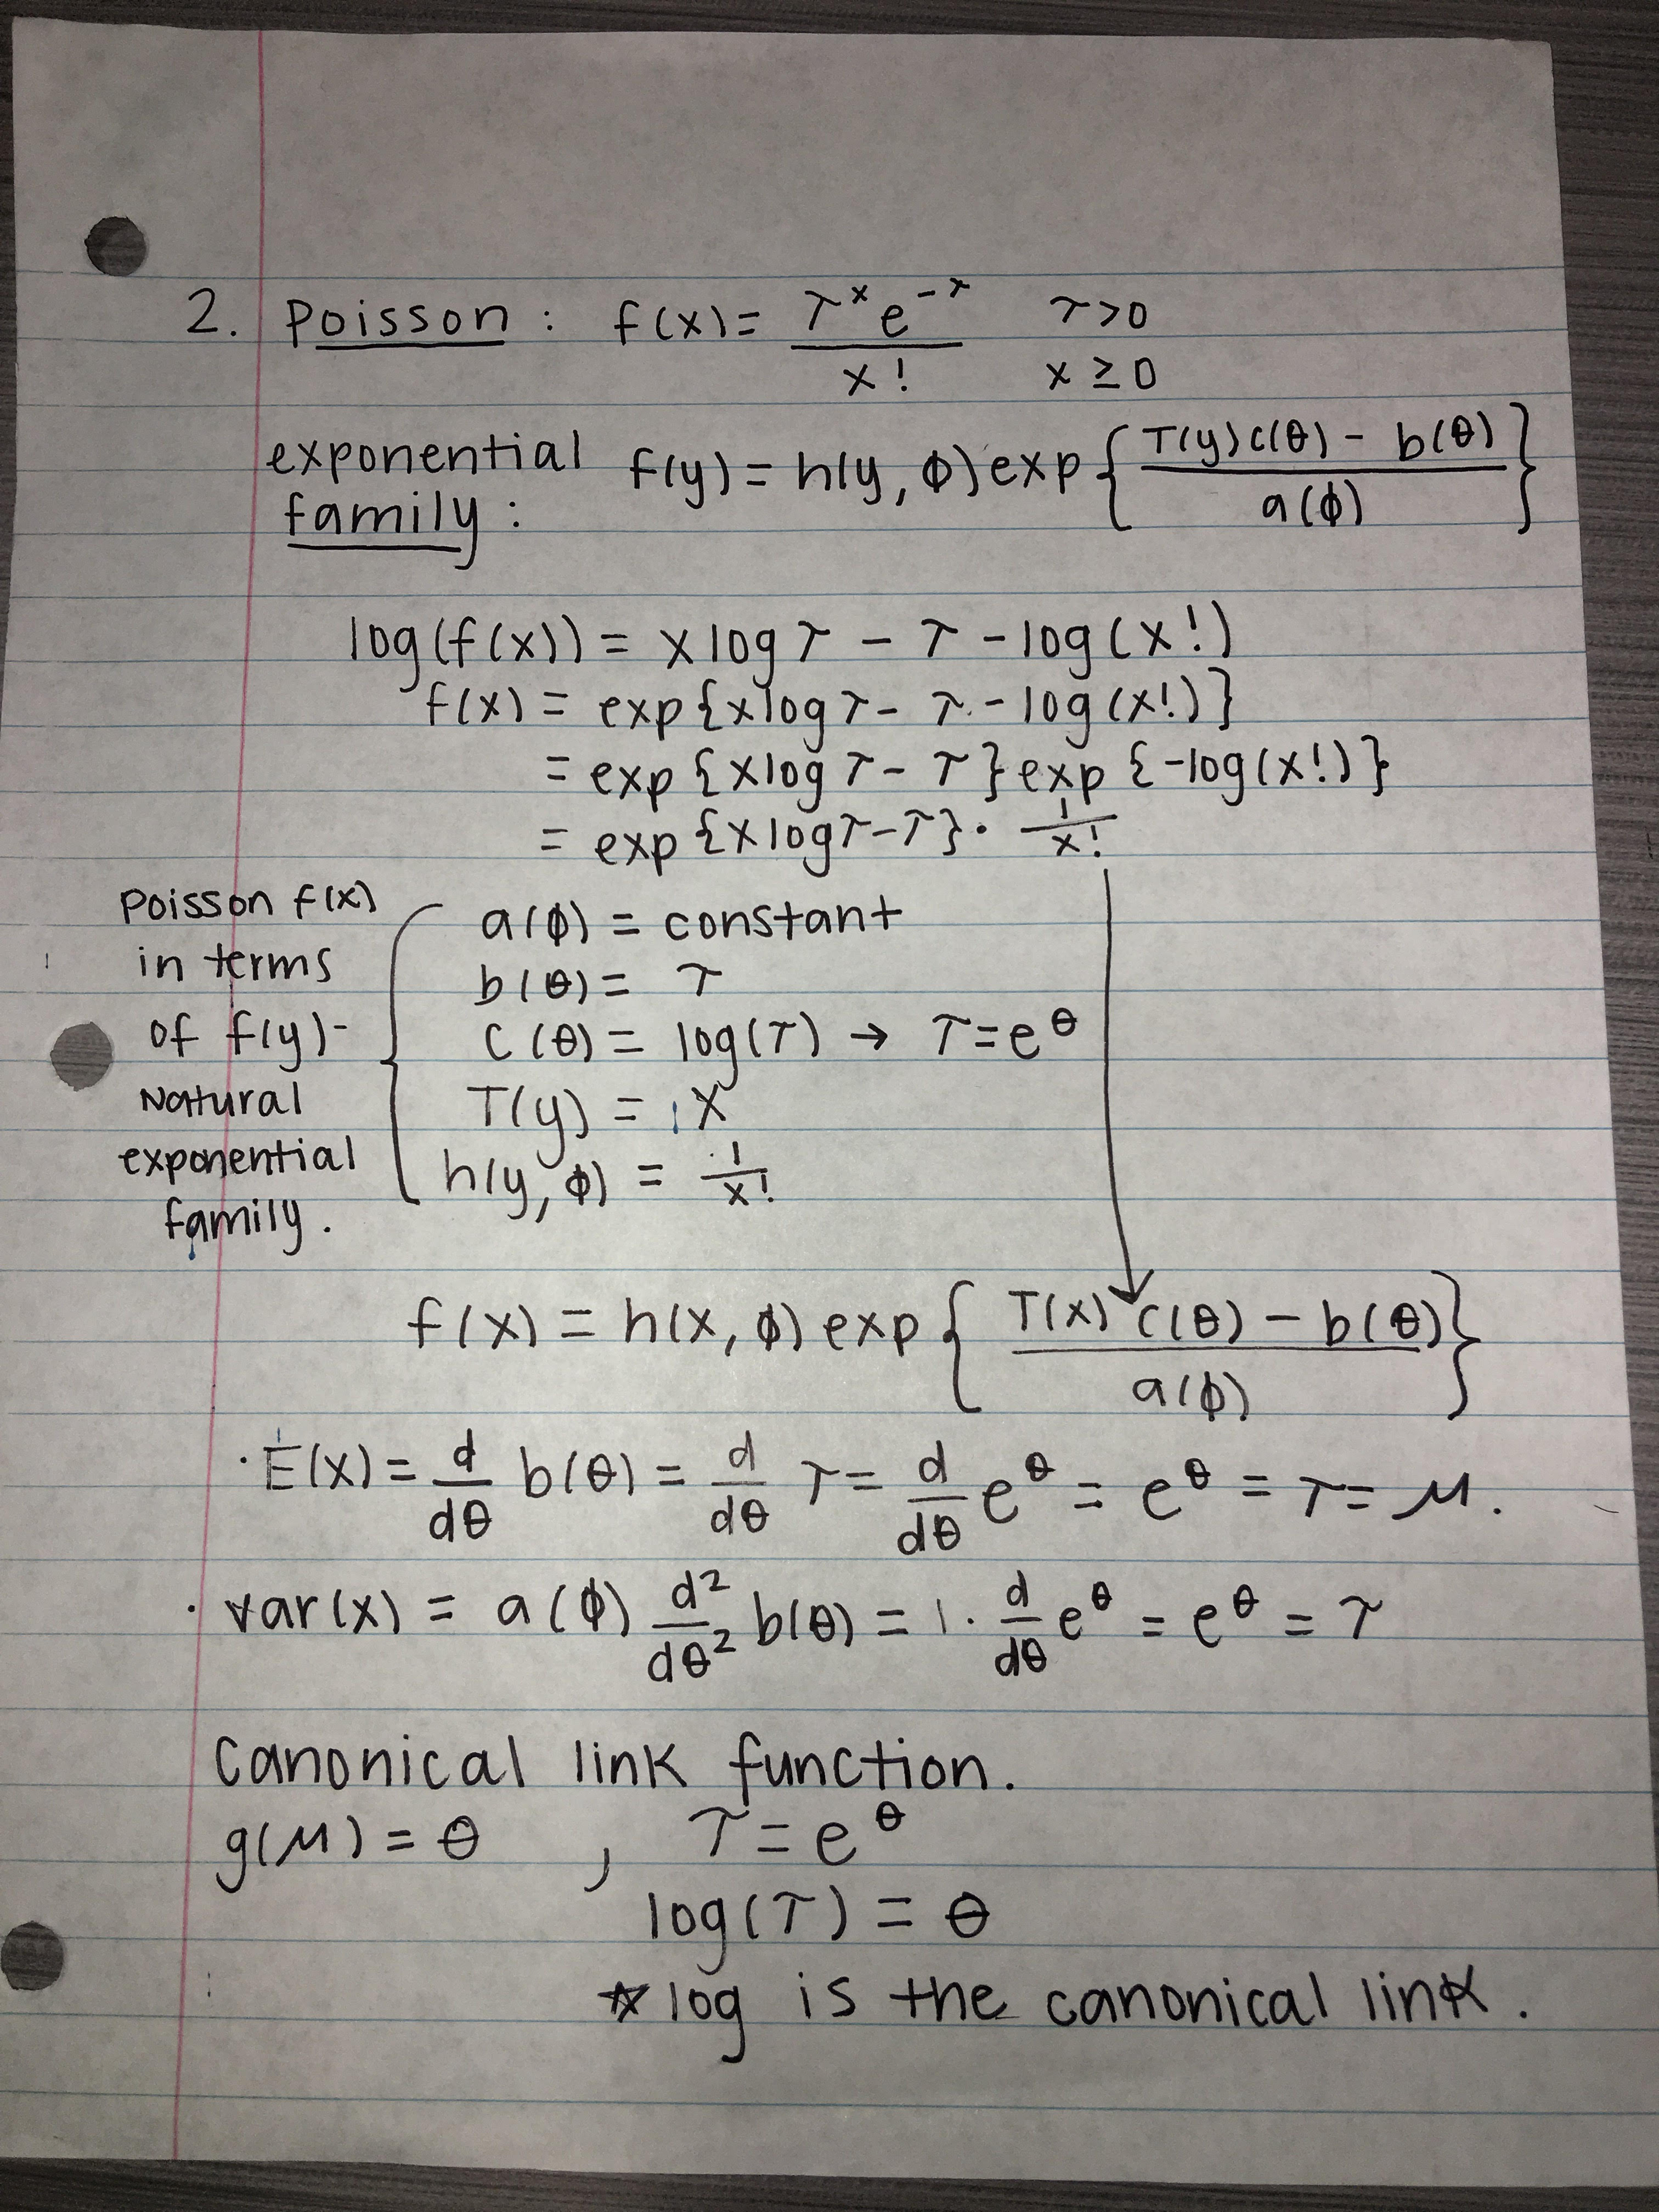
\includegraphics{/Users/JessKaminsky/glm_hw4/hw4_q2.jpg}
\caption{Question 2}
\end{figure}

\subsection{Question 3}\label{question-3}

The poisson iteratively reweighted least squares function that I have
written converges to the same values generated from the GLM function in
R using the poisson family. The only coefficent that differs slightly is
the one for the intercept term.

\begin{Shaded}
\begin{Highlighting}[]
\NormalTok{xa_test <-}\StringTok{ }\KeywordTok{data.matrix}\NormalTok{(}\KeywordTok{cbind}\NormalTok{(}\KeywordTok{rep}\NormalTok{(}\DecValTok{1}\NormalTok{,}\KeywordTok{nrow}\NormalTok{(risky)),risky[,(}\DecValTok{2}\NormalTok{:}\DecValTok{3}\NormalTok{)]))}
\NormalTok{ya_test <-}\StringTok{ }\NormalTok{risky[,}\DecValTok{6}\NormalTok{]}

\NormalTok{poisson_irls <-}\StringTok{ }\NormalTok{function(c, y, }\DataTypeTok{convergence =} \FloatTok{1e-20}\NormalTok{) \{}
  \NormalTok{diff =}\StringTok{ }\DecValTok{100}
  \NormalTok{b <-}\StringTok{ }\KeywordTok{rep}\NormalTok{(}\DecValTok{1}\NormalTok{, }\KeywordTok{ncol}\NormalTok{(c))}
  
  \NormalTok{while(}\KeywordTok{abs}\NormalTok{(diff)>convergence)\{}
    \NormalTok{eta =}\StringTok{ }\NormalTok{c %*%}\StringTok{ }\NormalTok{b}
    \NormalTok{mu =}\StringTok{ }\KeywordTok{exp}\NormalTok{(eta)}
    \NormalTok{theta =}\StringTok{ }\KeywordTok{log}\NormalTok{(mu) }\CommentTok{#theta = eta}
    \NormalTok{v =}\StringTok{ }\KeywordTok{exp}\NormalTok{(theta) }\CommentTok{# v = mu}
    \NormalTok{z =}\StringTok{ }\NormalTok{eta +}\StringTok{ }\NormalTok{(y -}\StringTok{ }\NormalTok{mu) *}\StringTok{ }\NormalTok{(}\DecValTok{1}\NormalTok{/mu)}
    \NormalTok{w =}\StringTok{ }\KeywordTok{ginv}\NormalTok{(v *}\StringTok{ }\NormalTok{((}\DecValTok{1}\NormalTok{/mu)^}\DecValTok{2}\NormalTok{))}
    
    \NormalTok{b_new =}\StringTok{ }\KeywordTok{ginv}\NormalTok{(}\KeywordTok{t}\NormalTok{(c) %*%}\StringTok{ }\KeywordTok{diag}\NormalTok{(}\KeywordTok{as.vector}\NormalTok{(w)) %*%}\StringTok{ }\NormalTok{c) %*%}\StringTok{ }\NormalTok{(}\KeywordTok{t}\NormalTok{(c) %*%}\StringTok{ }\KeywordTok{diag}\NormalTok{(}\KeywordTok{as.vector}\NormalTok{(w)) %*%}\StringTok{ }\NormalTok{z)}
    \NormalTok{diff =}\StringTok{ }\KeywordTok{sum}\NormalTok{(b_new -}\StringTok{ }\NormalTok{b)}
    \NormalTok{b =}\StringTok{ }\NormalTok{b_new}
  \NormalTok{\}}
  \NormalTok{b}
\NormalTok{\}}
\end{Highlighting}
\end{Shaded}

\subsubsection{Coefficients from Model in question A predicting fupacts
from couples and women alone indicator
variables}\label{coefficients-from-model-in-question-a-predicting-fupacts-from-couples-and-women-alone-indicator-variables}

\begin{Shaded}
\begin{Highlighting}[]
\NormalTok{model_a$coefficients}
\end{Highlighting}
\end{Shaded}

\begin{verbatim}
##  (Intercept)     couples1 women_alone1 
##    3.0895984   -0.3224256   -0.5721229
\end{verbatim}

\subsubsection{Coefficients generated using IRLS function with same
predictors and
output}\label{coefficients-generated-using-irls-function-with-same-predictors-and-output}

\begin{Shaded}
\begin{Highlighting}[]
\KeywordTok{poisson_irls}\NormalTok{(xa_test, ya_test)}
\end{Highlighting}
\end{Shaded}

\begin{verbatim}
##            [,1]
## [1,]  3.9841469
## [2,] -0.3224256
## [3,] -0.5721229
\end{verbatim}


\end{document}
